\documentclass[aspectratio=169]{beamer}

\usetheme{Madrid}
\usecolortheme{default}

% APCR Colors
\definecolor{apcrdarkblue}{RGB}{30,90,160}
\definecolor{apcrblue}{RGB}{60,140,230}
\definecolor{apcrlightblue}{RGB}{235,245,255}
\definecolor{accentorange}{RGB}{255,140,50}

% Apply colors to theme
\setbeamercolor{palette primary}{bg=apcrdarkblue,fg=white}
\setbeamercolor{palette secondary}{bg=apcrblue,fg=white}
\setbeamercolor{palette tertiary}{bg=apcrdarkblue,fg=white}
\setbeamercolor{palette quaternary}{bg=apcrblue,fg=white}
\setbeamercolor{structure}{fg=apcrdarkblue}
\setbeamercolor{section in toc}{fg=apcrdarkblue}
\setbeamercolor{subsection in head/foot}{bg=apcrlightblue,fg=apcrdarkblue}

% Remove navigation symbols
\setbeamertemplate{navigation symbols}{}

% Packages
\usepackage{graphicx}
\usepackage{booktabs}
\usepackage{listings}
\usepackage{tikz}
\usepackage{hyperref}

% Code listing style
\lstset{
    basicstyle=\ttfamily\footnotesize,
    keywordstyle=\color{apcrblue}\bfseries,
    commentstyle=\color{gray}\itshape,
    stringstyle=\color{accentorange},
    numbers=left,
    numberstyle=\tiny\color{gray},
    backgroundcolor=\color{white},
    showspaces=false,
    showstringspaces=false,
    showtabs=false,
    frame=single,
    rulecolor=\color{gray!30},
    tabsize=4,
    breaklines=true,
    language=Python
}

% Title page info
\title{A Deep Dive into Portfolio Optimisation}
\subtitle{Under the Hood}
\author{SCR Quantitative Research Team}
\institute{Surrey Capital Research, University of Surrey}
\date{January 2025}

\begin{document}

% Title slide
\begin{frame}
\titlepage
\end{frame}

% The Big Question
\begin{frame}{The Big Question}
\begin{center}
\Large
If you had \textbf{£100,000} to invest across\\
stocks, bonds, gold, and commodities...

\vspace{1em}

\textcolor{apcrblue}{\textbf{How would you split it?}}

\vspace{1em}

\normalsize
\begin{itemize}
    \item Split equally (1/18 per asset)?
    \item Use complex mathematical optimization?
    \item Something else?
\end{itemize}

\vspace{0.5em}
\textbf{We're testing this empirically.}
\end{center}
\end{frame}

% Research Question
\begin{frame}{The Research Question}
\begin{block}{Core Question}
Can sophisticated portfolio optimisation models beat the naive 1/N strategy?
\end{block}

\vspace{1em}

\textbf{Why this matters:}
\begin{itemize}
    \item \textbf{For investors:} Should you pay for complex portfolio management?
    \item \textbf{For students:} Does classroom theory work in practice?
    \item \textbf{For quant enthusiasts:} Rigorous empirical comparison
\end{itemize}

\vspace{0.5em}
\small
\textit{This is a live debate in quantitative finance — theory vs. practice.}
\end{frame}

% Investment Universe
\begin{frame}{Our Investment Universe}
\begin{table}
\centering
\begin{tabular}{l l r}
\toprule
\textbf{Asset Class} & \textbf{Examples} & \textbf{Count} \\
\midrule
UK Equities & HSBC, BP, Shell, Tesco, AstraZeneca, etc... & 15 \\
UK Government Bonds & iShares Core UK Gilts ETF & 1 \\
Precious Metals & Invesco Physical Gold ETC & 1 \\
Commodities & WisdomTree Commodities ETF & 1 \\
\midrule
\textbf{Total} & \textbf{Multi-Asset Portfolio} & \textbf{18} \\
\bottomrule
\end{tabular}
\end{table}

\vspace{0.5em}

\textbf{Data period:} 2015–2025 (10 years)
\begin{itemize}
    \item Includes COVID crash, 2022 selloff, Brexit volatility
    \item Daily prices, monthly rebalancing
\end{itemize}
\end{frame}

% The Models - Overview
\begin{frame}{The Four Strategies We're Testing}
\begin{enumerate}
    \item \textbf{Equal Weight (1/N)} — Naive baseline
    \vspace{0.3em}
    \item \textbf{Mean-Variance Optimisation (MVO)} — Markowitz (1952)
    \vspace{0.3em}
    \item \textbf{Black-Litterman} — Bayesian equilibrium + views
    \vspace{0.3em}
    \item \textbf{Risk Parity} — Equal risk contribution
\end{enumerate}

\vspace{1em}
\begin{center}
\textcolor{apcrblue}{\textbf{All tested on identical data with identical methodology}}
\end{center}
\end{frame}

% Model 1: Equal Weight
\begin{frame}{Strategy 1: Equal Weight (1/N)}
\begin{block}{The Benchmark}
Simplest possible: split money equally across all 18 assets
\end{block}

\textbf{How it works:}
\begin{itemize}
    \item £5,556 to each asset (on £100k capital)
    \item Monthly rebalancing to maintain 1/18 weights
    \item No forecasting, no optimization
\end{itemize}

\vspace{0.5em}

\begin{alertblock}{Why it's tough to beat}
DeMiguel et al. (2009): Equal weight often beats sophisticated models due to estimation error in expected returns and covariances.
\end{alertblock}
\end{frame}

% Model 2: MVO
\begin{frame}{Strategy 2: Mean-Variance Optimisation}
\begin{block}{Markowitz (1952) — Foundation of Modern Portfolio Theory}
Maximize return for given risk (or minimize risk for given return)
\end{block}

\vspace{0.5em}

\textbf{Optimization:}
\[
\max_{w} \frac{w^T \mu - r_f}{\sqrt{w^T \Sigma w}} \quad \text{s.t.} \quad \sum w_i = 1, \, w_i \geq 0
\]

\vspace{0.5em}

\textbf{The challenge:}
\begin{itemize}
    \item Very sensitive to estimation errors in $\mu$ and $\Sigma$
    \item Small input changes → big portfolio changes
    \item Can produce extreme, unstable weights
\end{itemize}
\end{frame}

% Model 3: Black-Litterman
\begin{frame}{Strategy 3: Black-Litterman}
\begin{block}{Combining Market Equilibrium with Investor Views}
Overcomes MVO instability by anchoring to market equilibrium
\end{block}

\textbf{How it works:}
\begin{enumerate}
    \item Start with equilibrium returns (from market cap weights)
    \item Express views: "UK banks will outperform by 2\%"
    \item Blend equilibrium + views using Bayesian updating
    \item Optimize portfolio with posterior returns
\end{enumerate}

\vspace{0.5em}

\textbf{Key advantage:} More stable than pure MVO — doesn't require perfect forecasts
\end{frame}

% Model 4: Risk Parity
\begin{frame}{Strategy 4: Risk Parity}
\begin{block}{Equal Risk Contribution, Not Equal Capital}
Philosophy: diversify risk, not just money
\end{block}

\vspace{0.5em}

Each asset contributes equally to total portfolio risk:
\[
w_i \times \frac{\partial \sigma_p}{\partial w_i} = \frac{\sigma_p}{N}
\]

\vspace{0.5em}

\textbf{In practice:}
\begin{itemize}
    \item Bonds (low vol) get \textit{more} capital
    \item Equities (high vol) get \textit{less} capital
    \item Popular with institutional investors (e.g., Bridgewater All Weather)
\end{itemize}
\end{frame}

% Backtesting Methodology
\begin{frame}{How We're Testing: Backtesting Engine}
\begin{center}
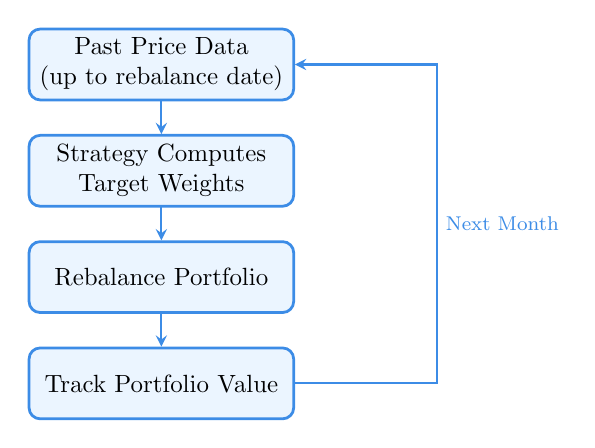
\begin{tikzpicture}[node distance=1.5cm, scale=0.9, every node/.style={scale=0.9}]
    \tikzstyle{block} = [rectangle, draw, fill=apcrlightblue,
        text width=3.5cm, text centered, rounded corners=4pt, minimum height=1cm,
        line width=1pt, draw=apcrblue]
    \tikzstyle{arrow} = [thick,->,>=stealth,color=apcrblue]

    \node [block] (data) {Past Price Data\\(up to rebalance date)};
    \node [block, below of=data] (strategy) {Strategy Computes\\Target Weights};
    \node [block, below of=strategy] (rebalance) {Rebalance Portfolio};
    \node [block, below of=rebalance] (track) {Track Portfolio Value};

    \draw [arrow] (data) -- (strategy);
    \draw [arrow] (strategy) -- (rebalance);
    \draw [arrow] (rebalance) -- (track);
    \draw [arrow] (track.east) -- ++(2,0) |- node[near start, right, font=\footnotesize] {Next Month} (data.east);
\end{tikzpicture}
\end{center}

\vspace{0.3em}

\begin{alertblock}{Critical: No Look-Ahead Bias}
Strategies only see \textbf{past data}. This prevents unrealistically good backtest results.
\end{alertblock}
\end{frame}

% Code: Look-Ahead Bias Prevention
\begin{frame}[fragile]{Code: Preventing Look-Ahead Bias}
\begin{lstlisting}
for current_date in dates:
    if current_date in rebalance_dates:
        # CRITICAL: Only past data
        past_prices = self.prices.loc[:current_date]

        # Strategy uses ONLY past data
        target_weights = self.strategy.get_target_weights(
            decision_date=current_date,
            past_prices=past_prices  # No future!
        )

        # Execute rebalancing
        # ...

    # Track portfolio value
    equity_curve[current_date] = portfolio_value
\end{lstlisting}
\end{frame}

% Performance Metrics
\begin{frame}{What We're Measuring}
\begin{table}
\small
\begin{tabular}{l p{7cm}}
\toprule
\textbf{Metric} & \textbf{What It Measures} \\
\midrule
Total Return & Cumulative gain/loss over 10 years \\
CAGR & Annualised return \\
Volatility & Annualised standard deviation \\
Sharpe Ratio & Excess return per unit of risk \\
Max Drawdown & Worst peak-to-trough loss \\
Sortino Ratio & Return per unit of downside risk \\
Turnover & Trading frequency (costs) \\
\bottomrule
\end{tabular}
\end{table}

\vspace{0.5em}
\textbf{Goal:} Understand risk-adjusted performance, not just returns
\end{frame}

% What Insights We Expect
\begin{frame}{What Insights We're Looking For}
\textbf{1. Risk-Adjusted Performance}
\begin{itemize}
    \item Which model has the best Sharpe ratio?
    \item Is complexity worth the cost?
\end{itemize}

\vspace{0.5em}

\textbf{2. Crisis Performance}
\begin{itemize}
    \item COVID crash (March 2020)
    \item 2022 equity-bond selloff
    \item Brexit volatility (2016)
\end{itemize}

\vspace{0.5em}

\textbf{3. Practical Considerations}
\begin{itemize}
    \item Turnover costs
    \item Implementation difficulty
    \item Robustness to parameter choices
\end{itemize}
\end{frame}

% Strategy Architecture
\begin{frame}[fragile]{The Strategy Architecture}
\small
\begin{block}{BaseStrategy Interface}
All models implement this clean abstraction:
\end{block}

\begin{lstlisting}
class BaseStrategy(ABC):
    @abstractmethod
    def get_target_weights(
        self,
        decision_date: pd.Timestamp,
        past_prices: pd.DataFrame,  # ONLY past
        current_positions: pd.Series,
        cash: float,
    ) -> pd.Series:
        """Return target weights (sum = 1.0)"""
        raise NotImplementedError
\end{lstlisting}

\textbf{Why?} Fair comparison, extensibility, enforces no look-ahead bias
\end{frame}

% Example: Equal Weight Implementation
\begin{frame}[fragile]{Example: Equal Weight Strategy}
\begin{lstlisting}
class EqualWeightStrategy(BaseStrategy):
    def __init__(self, tickers: list[str]):
        self.tickers = tickers

    def get_target_weights(self, decision_date,
                          past_prices,
                          current_positions, cash):
        # Just return 1/N for all assets
        n = len(self.tickers)
        weights = pd.Series(1.0 / n,
                           index=self.tickers)
        return weights
\end{lstlisting}

\vspace{0.3em}
\begin{center}
\textcolor{apcrblue}{\textbf{Simple, but surprisingly hard to beat!}}
\end{center}
\end{frame}

% Progress Update
\begin{frame}{Where We Are Now}
\begin{columns}
\begin{column}{0.48\textwidth}
\textbf{Completed:}
\begin{itemize}
    \item Data pipeline (18 assets, 2015-2025)
    \item Backtesting engine
    \item Equal weight baseline
    \item Black-Litterman framework
\end{itemize}
\end{column}

\begin{column}{0.48\textwidth}
\textbf{→ In Progress:}
\begin{itemize}
    \item MVO implementation
    \item Black-Litterman views
    \item Risk Parity solver
    \item Performance analysis
\end{itemize}
\end{column}
\end{columns}

\vspace{1em}

\begin{block}{Coming Soon}
\begin{itemize}
    \item Full backtest results across all 4 strategies
    \item Regime analysis (bull/bear/crisis)
    \item Comprehensive research report
\end{itemize}
\end{block}
\end{frame}

% What This Research Means
\begin{frame}{What This Means}
\begin{center}
\Large
\textcolor{apcrdarkblue}{\textbf{Bridging the gap between theory and practice}}
\end{center}

\vspace{1em}

\begin{itemize}
    \item \textbf{For investors:} Does sophisticated management add value?
    \vspace{0.5em}
    \item \textbf{For students:} Testing what you learn in lectures
    \vspace{0.5em}
    \item \textbf{For quants:} Rigorous comparison with clean methodology
\end{itemize}

\vspace{1em}

\begin{center}
\textit{Academic finance says "here's the optimal solution"\\
We're asking: "does it actually work?"}
\end{center}
\end{frame}

% Follow Along
\begin{frame}{Want to Follow Along?}
\begin{center}
\Large
\textbf{GitHub Repository}\\
\vspace{0.5em}
\normalsize
\url{github.com/AP-Capital-Research/deep-dive-into-portfolio-optimisation}

\vspace{2em}

\Large
\textbf{Full Research Report}\\
\vspace{0.5em}
\normalsize
Expected publication: [Month] 2025

\vspace{2em}

\textbf{Questions or feedback?}\\
Contact us at [email/contact]
\end{center}
\end{frame}

% Thank You
\begin{frame}
\begin{center}
\Huge
\textcolor{apcrdarkblue}{\textbf{Thank You}}

\vspace{2em}

\Large
We're excited to share our findings\\
with the quant finance community

\vspace{1em}

\normalsize
\textit{Stay tuned for the full results}
\end{center}
\end{frame}

\end{document}
